# Introducción

## Presentación del curso

### Presentaciones

* \subsubtitle{Estudiantes}
    - \subsubtitleC{Conocimientos previos.}
    - \subsubtitleC{Experiencia profesional.}
    \pause
* \subsubtitle{Profesor:}
    \pause

    \vspace{-6mm}
    \begin{center}
    \hspace{20mm}\begin{customRoundedBox}{}
    \centering
        \subsubtitle{Nicolás Eugenio Ozimica}\\
        \vspace{4mm}
        \subsubtitleC{Ingeniero Civil en Computación}\\
        \subsubtitleC{Universidad de Chile}
    \end{customRoundedBox}
    
    \hspace{60mm}\begin{customRoundedBox}{}
    \centering
        \subsubtitleC{nozimica@dcc.uchile.cl}\\
        \subsubtitleC{nozimica@gmail.com}
    \end{customRoundedBox}
    \end{center}

### Objetivos del Curso

- Dominar el paradigma de programación orientada a objetos, desde un punto de vista 
  práctico, apoyado en un adecuado marco teórico.
  \pause
- Modelar una arquitectura de \itt{e-business} utilizando orientación a objetos
  con el objetivo de apoyar los procesos de negocio
  de una empresa u organización.
  \pause
- Como herramienta en la ilustración de este modelo se utilizará los diagramas UML.
  \pause
- Analizar el modelo de datos subyacente.
  \pause
- Lo teórico sólo se domina a través de la práctica: 
    - Implementar algunos de nuestros diseños en un lenguaje de programación real: Java o Python.

### Actividades

- Clases teóricas los días sábado:
    - Horario: 8:30 a 11:45.
    - Horario alternativo: 9:00 a 12:15.

- Clases auxiliares:
    - Horario por definir.

- Evaluaciones:
    - Controles, tareas y proyectos:
        - Cantidad y fechas por definir.
    - Examen individual.
        - Última clase de cátedra.


### Contenido del curso

1. Conceptos básicos de la Orientación a Objetos (OO).
1. Arquitectura tecnológica y de software.
1. Requisitos de software.
1. Modelamiento orientado a objetos con UML.
    - Diagramas de Casos de Uso.
    - Diagramas de Secuencias.
    - Modelo de clases, objetos y componentes.
    - Modelamiento de los datos.
1. Modelamiento de la arquitectura de software.
    - Modelo de componentes del e-business.
    - Modelos UML para entrega y distribución.
1. Relación con la arquitectura de un *e-business*.

### Bibliografía

\nocite{*}
\bibliographystyle{apalike}
{\scriptsize
\bibliography{bibliog}}

# Conceptos básicos de la OOP.

### Conceptos básicos de la OOP.

- Sin **Lenguajes de programación** no hay aplicaciones.

\pause
\vfill

- Son muy importantes, pues nos permiten implementar las lógicas de la aplicación.

\pause
\vfill

- Hay formas muy distintas de programar una aplicación: 
    - Lógica.
    - Funcional.
    - Imperativa o Procedural.
    - Orientada a Objetos.

### Programación imperativa

- Planteamos nuestro algoritmo como un conjunto de subprocesos, los cuales manipulan los datos
de la aplicación.

\pause \vfill

- Entre los más importantes lenguajes imperativos tenemos:
    - BASIC
    - Pascal
    - C
    - Fortran

### Programación imperativa vs OOP

- En la programación imperativa, los datos se encuentran separados de los subprocesos.\vfill
- En OOP, los datos y los subprocesos están integrados en las clases.

\centering\begin{tikzflowchart}
  \node (a1) [startstop, text width=40mm] {Las clases son el núcleo de la OOP.};
\end{tikzflowchart}
\vfill

- **Concepto importantísimo**: La OOP es una herramienta que nos permite diseñar modelos
reutilizables.

\centering\begin{tikzflowchart}
  \node (a1) [startstop, text width=40mm] {¿Para qué volver a inventar la rueda?};
\end{tikzflowchart}

- Y junto con ser reutilizables, también son mantenibles más fácilmente.

### Programación imperativa vs OOP

- Pero el paradigma imperativo no es tan opuesto al orientado a objetos:
    - Por lo general, un lenguaje OOP se puede utilizar ---con mayor o menor dificultad--- como
    si fuera solamente imperativo (pero no al revés).

- Ejemplos más claros:
    - C++
    - Java
    - Python

- Hay otros lenguajes que empezaron como imperativos, y con el tiempo fueron extendidos
para ser compatibles con OOP:
    - PHP4 vs PHP5

### Lenguajes OOP destacados

**C++**

- C++ (1983) fue desarrollado en *Bell Laboratories* por Bjarne Stroustrup.
- Influenciado por C y Simula.
- Lenguaje orientado a objetos híbrido, compatible con C (no al revés).
- Soporta clases, encapsulación, sobrecarga de funciones y operadores, herencia múltiple, polimorfismo, clases/funciones parametrizadas (genéricas).


### Lenguajes OOP destacados {.fragile}

**C++**\vfill

Un ejemplo de un código simple:
\begin{lstlisting}[language=C++]
#include <iostream>

void main()
{
    std::cout << "Hello, world!" << std::endl;
}
\end{lstlisting}

- Si bien es C++, este código se tan simple que no es OOP.

### Lenguajes OOP destacados

**Java**

- Java (1995) fue desarrollado en *Sun Microsystems* por James Gosling, Bill Joy y Guy Steele.
- Influenciado por C++.
- Java es un lenguaje orientado a objetos más puro que C++ y menos puro que Smalltalk.
- Soporta clases, encapsulación, herencia simple, polimorfismo, interfaces, garbage collection.

### Lenguajes OOP destacados

**Java**

- Objetivo inicial: un lenguaje de programación para dispositivos de consumo.
- Requerimientos: pequeño, rápido, confiable y portable.
- En 1994 se produce la explosión del Web y Sun advierte que Java es ideal para aplicaciones Internet:
    - Independiente de la plataforma.
    - Pequeño.
    - Seguro.

### Lenguajes OOP destacados {.fragile}

**Java**\vfill

Un ejemplo de un código simple:
\begin{lstlisting}[language=Java]
public class HelloWorld {
    public static void main(String() args) {
        System.out.println("Hello, world!");
    }
}
\end{lstlisting}

- Java, por muy simple que sea el programa, siempre se implementa en OOP.

### Lenguajes OOP destacados

**PHP**

- ¿Qué significa PHP?
    - Es un acrónimo recursivo: *PHP: Hypertext Preprocessor*.
- Es un lenguaje de código abierto muy popular especialmente adecuado para el desarrollo web y que puede ser incrustado en HTML. 
- Se ejecuta dentro del servidor web.
    - Ejecuta el código PHP.
    - Genera código HTML.
    - El navegador del usuario recibe ese código, desplegándolo como una página web.
- Es extremadamente simple para principiantes en la programación.
    - Usado adecuadamente, puede ser muy poderoso.

### Lenguajes OOP destacados {.fragile}

**PHP**\vfill

Un ejemplo de un código simple:
\begin{lstlisting}[language=PHP]
<html>
 <head>
  <title>Prueba de PHP</title>
 </head>
 <body>
 <?php echo '<p>Hola Mundo</p>'; ?>
 </body>
</html>
\end{lstlisting}

- Este es un código simple, y de un estilo **no recomendable** de programación en PHP.
    - Mezcla HTML con PHP: desordenado y poco mantenible.
    - Pero es el primer y más sencillo ejemplo.
    - De hecho, es el que está en el tutorial oficial de PHP.

### Programación Orientada a Objetos

- Según Grady Booch:\vspace{7mm}

    - ``La Programación Orientada a Objetos es un método de implementación en el que los programas se organizan como **colecciones de objetos**, cada uno de los cuales representa una **instancia de alguna clase**, y cuyas clases pertenecen a una jerarquía.''\vspace{10mm}
    - ``Un objeto tiene **estado**, exhibe algún **comportamiento bien definido**, y tiene una **identidad única**.''

### Programación Orientada a Objetos

- Es un enfoque diferente.\vfill

- Se basa en abstracciones de la realidad:

\centering\begin{tikzflowchart}
  \node (a1) [startstop, text width=40mm] {Conceptos en el mundo real.};
  \node (a2) [startstop, right=15mm of a1, text width=40mm] {Conceptos del modelo.};
  \draw [arrow] (a1) -- (a2);
\end{tikzflowchart}
\vfill

- Modela el problema a resolver como un grupo de **objetos**.\vfill
- Lo normal es que existan diversos tipos de objetos: **clases**.\vfill
- Los objetos tienen **características** propias.\vfill
- Estos objetos **interactúan** entre sí por medio de mensajes.\vfill

### Qué es la OOP

**Concepto clave:**

- Objetos:
    - Son el centro de la OOP.

\centering\begin{tikzpicture}
\node[inner sep=0pt] (house) at (0,0)
{
\includegraphics[width=20mm]{icons/326-emoji_android_house_building.png}};
\node[inner sep=0pt] (person) at (4,0)
{
\includegraphics[width=20mm]{icons/450-emoji_android_dancer.png}};
\node[inner sep=0pt] (bank) at (8,0)
{
\includegraphics[width=20mm]{icons/331-emoji_android_bank.png}};

\node (a1) [process, below=10mm of house, text width=15mm] {Casa};
\node (a2) [process, below=10mm of person, text width=15mm] {Persona};
\node (a3) [process, below=10mm of bank, text width=15mm] {Banco};

\draw[->,thick] (a2) -- (a1)
  node[namedArrow] {{\scriptsize \phantom{j} vive en}};
\draw[->,thick] (a2) -- (a3)
  node[namedArrow] {{\scriptsize trabaja en}};
\end{tikzpicture}

### Qué es la OOP

**Concepto clave:**

- Objetos:
    - Tienen propiedades:

\centering\begin{tikzpicture}
\node[inner sep=0pt] (elephant) at (0,0)
{
\includegraphics[width=20mm]{icons/349-emoji_android_elephant.png}};

\node (c1) [feature, right=18mm of elephant, text width=25mm] {Color};
\node (c2) [feature, above=3mm of c1, text width=25mm] {Peso};
\node (c3) [feature, above=3mm of c2, text width=25mm] {Sexo};
\node (c4) [feature, below=3mm of c1, text width=25mm] {Edad};
\node (c5) [feature, below=3mm of c4, text width=25mm] {Hábitat};

\draw[->,thick] (elephant) -- (c1.west);
\draw[->,thick] (elephant) -- (c2.west);
\draw[->,thick] (elephant) -- (c3.west);
\draw[->,thick] (elephant) -- (c4.west);
\draw[->,thick] (elephant) -- (c5.west);
\end{tikzpicture}

### Qué es la OOP

**Concepto clave:**

- Objetos:
    - Ejecutan acciones:

\centering\begin{tikzpicture}
\node[inner sep=0pt] (horse) at (0,0)
{
\includegraphics[width=20mm]{icons/344-emoji_android_horse.png}};

\node (c1) [methods, right=18mm of horse, text width=25mm] {Galopar};
\node (c2) [methods, above=3mm of c1, text width=25mm] {Dormir};
\node (c3) [methods, above=3mm of c2, text width=25mm] {Mirar};
\node (c4) [methods, below=3mm of c1, text width=25mm] {Comer};
\node (c5) [methods, below=3mm of c4, text width=25mm] {Saltar};

\draw[->,thick] (horse) -- (c1.west);
\draw[->,thick] (horse) -- (c2.west);
\draw[->,thick] (horse) -- (c3.west);
\draw[->,thick] (horse) -- (c4.west);
\draw[->,thick] (horse) -- (c5.west);
\end{tikzpicture}

### Qué es la OOP

**Concepto clave:**

- Objetos:
    - Representan a un elemento del mundo real.
\begin{center}\begin{tikzpicture}
\node[inner sep=0pt] (elephant) at (0,0)
{
\includegraphics[width=10mm]{icons/349-emoji_android_elephant.png}};
\node[inner sep=0pt] (horse) at (2,0)
{
\includegraphics[width=10mm]{icons/344-emoji_android_horse.png}};
\node[inner sep=0pt] (house) at (4,0)
{
\includegraphics[width=10mm]{icons/326-emoji_android_house_building.png}};
\end{tikzpicture}\end{center}
    - Considera sus características y estados relevantes.
\begin{center}\begin{tikzflowchart}
  \node (a1) [startstop, text width=40mm] {Propiedades};
\end{tikzflowchart}\end{center}
    - Modela su comportamiento.
\begin{center}\begin{tikzflowchart}
  \node (a1) [startstop, text width=40mm] {Métodos};
\end{tikzflowchart}\end{center}


### Qué es la OOP: métodos

**Métodos de un objeto**:

- Pueden ser de dos tipos:
    - Métodos públicos (de interfaz): son las acciones relevantes para el exterior del objeto.
    - Métodos privados (internos): comportamiento interno del objeto.

\begin{center}\begin{tikzpicture}[font=\sffamily\scriptsize]
\tikzstyle{roundComment} = [ellipse, fill=white, draw=black!10, aspect=2, text width=25mm, align=center]
\node[inner sep=0pt] (truck) at (0,0)
{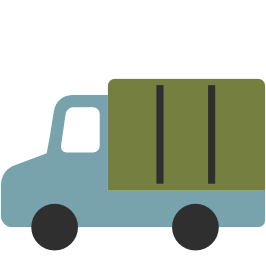
\includegraphics[width=20mm]{icons/703-emoji_android_delivery_truck.png}};
\node (c1) [methods, left=13mm of truck, text width=25mm] {Encender\\camión};
\node (c2) [methods, right=13mm of truck, text width=25mm] {Prender motor de arranque};
\draw[->,thick] (truck) -- (c1.east)
  node[namedArrow] {{\scriptsize público}};
\draw[->,thick] (truck) -- (c2.west)
  node[namedArrow] {{\scriptsize privado}};

\node[roundComment, below=8mm of c1] (cloudpublic) {\tiny Utilizado por\\el conductor};
\node[roundComment, below=8mm of c2] (cloudprivate) {\tiny No es necesario\\prenderlo manualmente};
\draw[->,dotted] (cloudpublic) -- (c1.south);
\draw[->,dotted] (cloudprivate) -- (c2.south);
\end{tikzpicture}\end{center}

### Qué es la OOP: métodos

**Métodos de un objeto**:

- La posibilidad de diferenciar métodos públicos de privados es una herramienta muy poderosa.
- Permite un mejor control del uso del objeto por parte de los otros objetos.
- Permite reflejar más fielmente la realidad.
- Se puede modificar el diseño **interno** de un objeto, sin exponer ese cambio hacia el exterior.

